\chapter{Inclusive CLFV Signals}
\label{chap:Signal}

\section{Targeted Signals}
\label{sec:Target}

 \begin{figure}[tbh!]
 \begin{center}
 \begin{tabular}{ccc}
 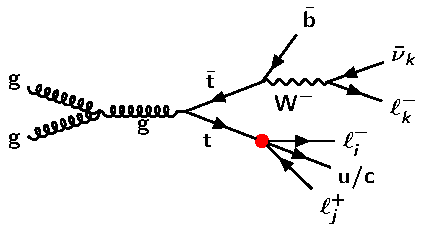
\includegraphics[width=0.33\textwidth]{figures/Part4/Signal/TT}&
 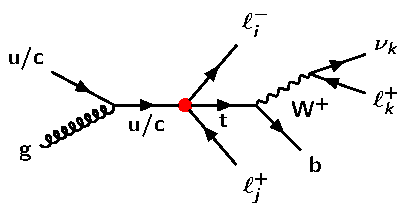
\includegraphics[width=0.33\textwidth]{figures/Part4/Signal/ST1}&
 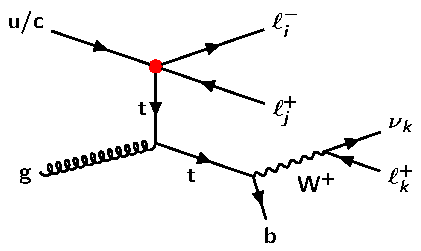
\includegraphics[width=0.33\textwidth]{figures/Part4/Signal/ST2}\\
 \end{tabular}
 \caption{Representative Feynman diagrams for the signal processes that are targeted by this analysis. Both top quark decay (left) and production (middle and right) \ac{CLFV} processes are shown. The indices $i$,  $j$, and $k$ are lepton flavor indices that run from 1 to 3 with the following conditions: i) $i\neq j$, ii) one of these three indices is 3, and iii) the other two are smaller than 3.}
 \label{fig:Target}
 \end{center}
 \end{figure}

\section{Signal Event Generation}
\label{sec:SigGen}

 \begin{figure}[tbh!]
 \begin{center}
 \begin{tabular}{ccc}
 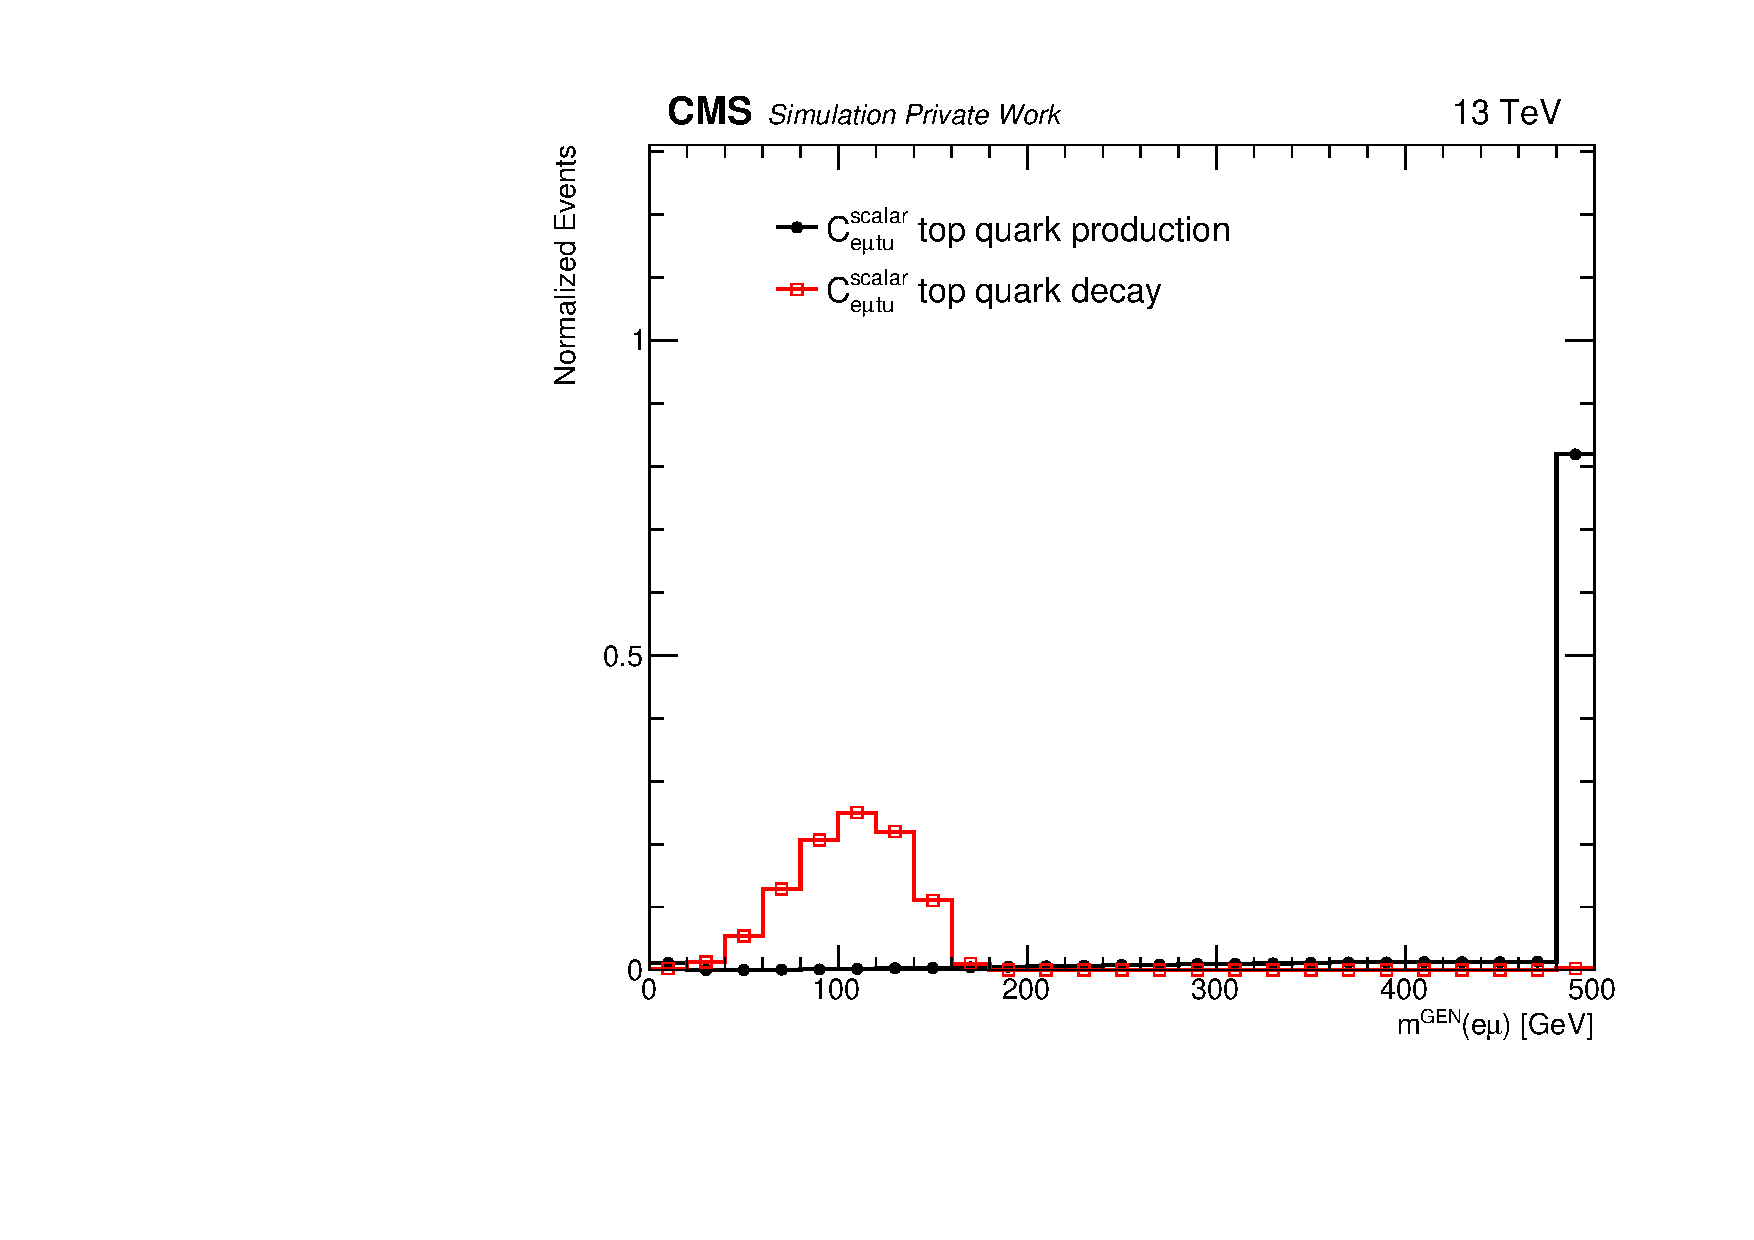
\includegraphics[width=0.33\textwidth]{figures/Part4/Signal/llM_emu}&
 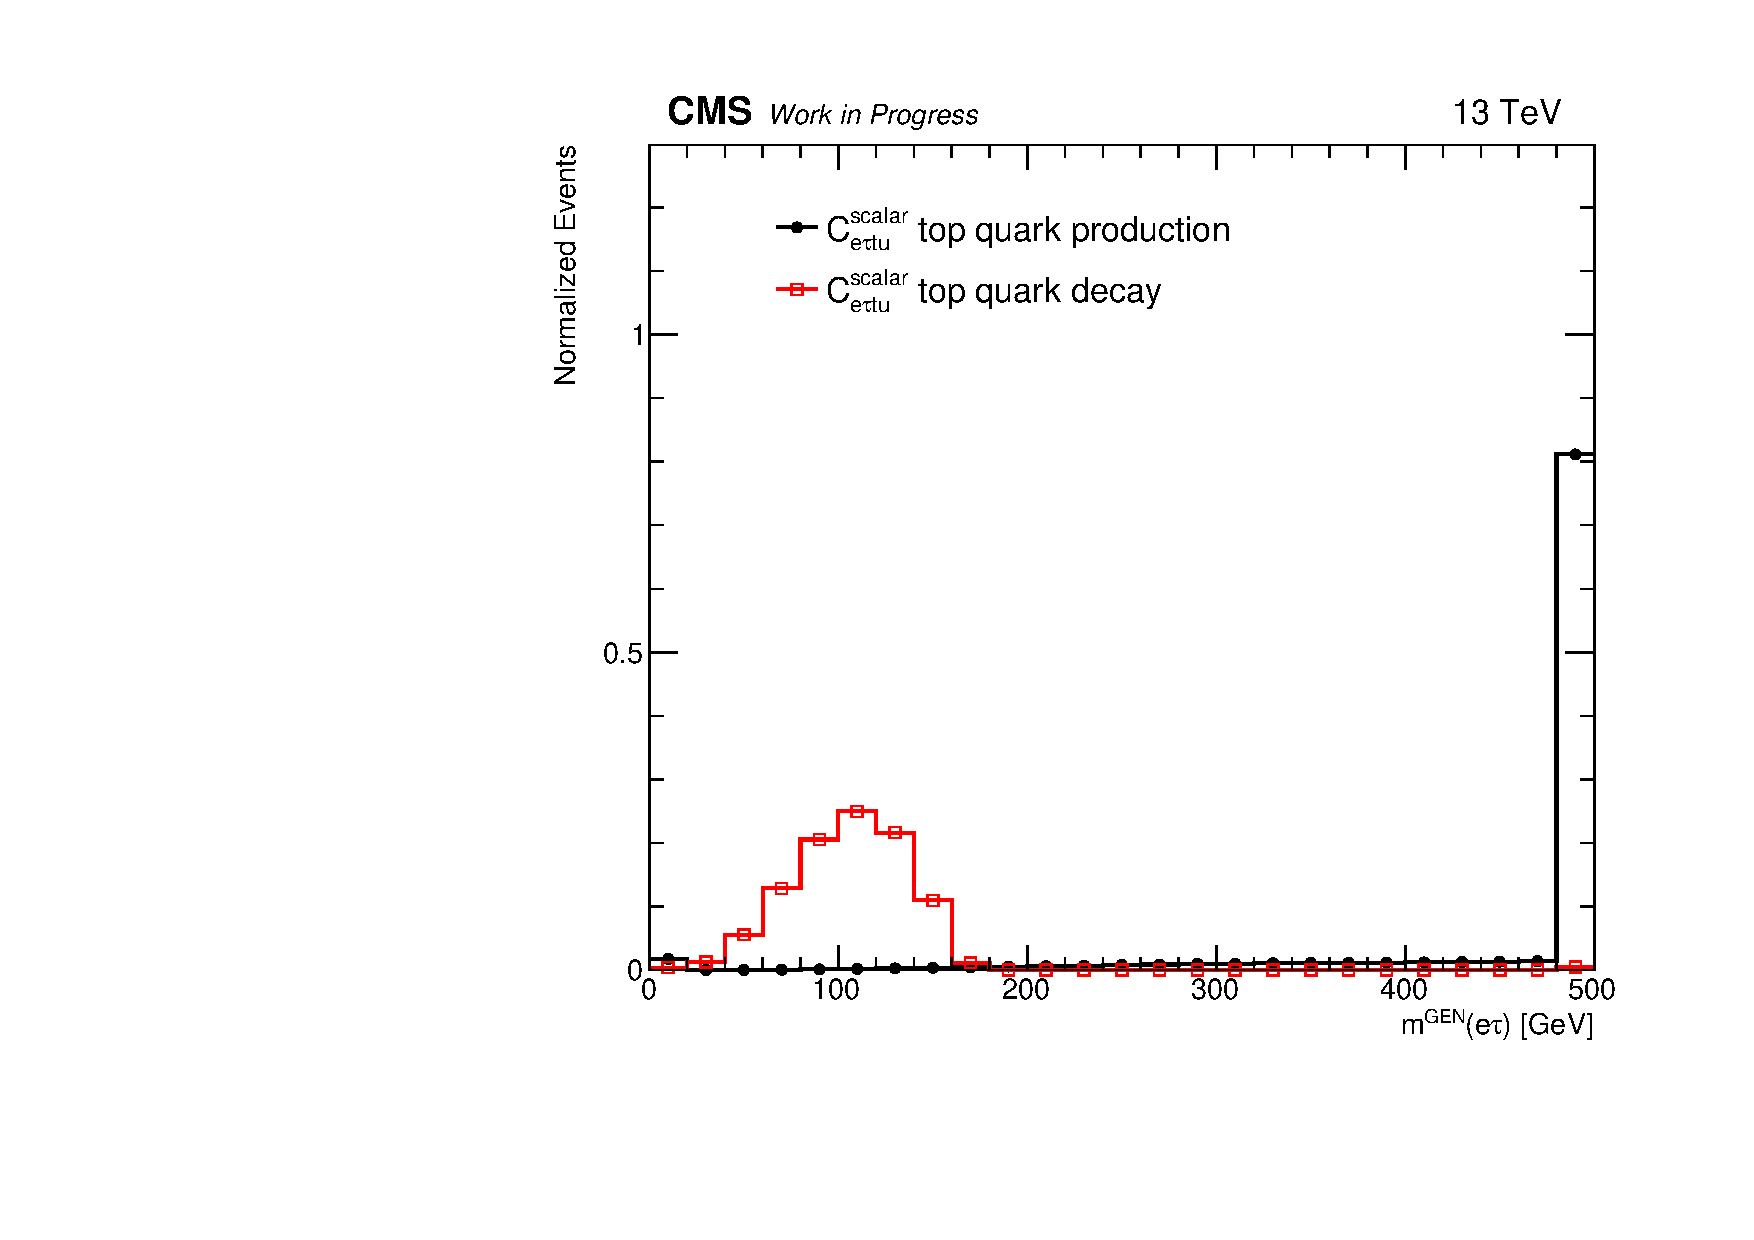
\includegraphics[width=0.33\textwidth]{figures/Part4/Signal/llM_etau}&
 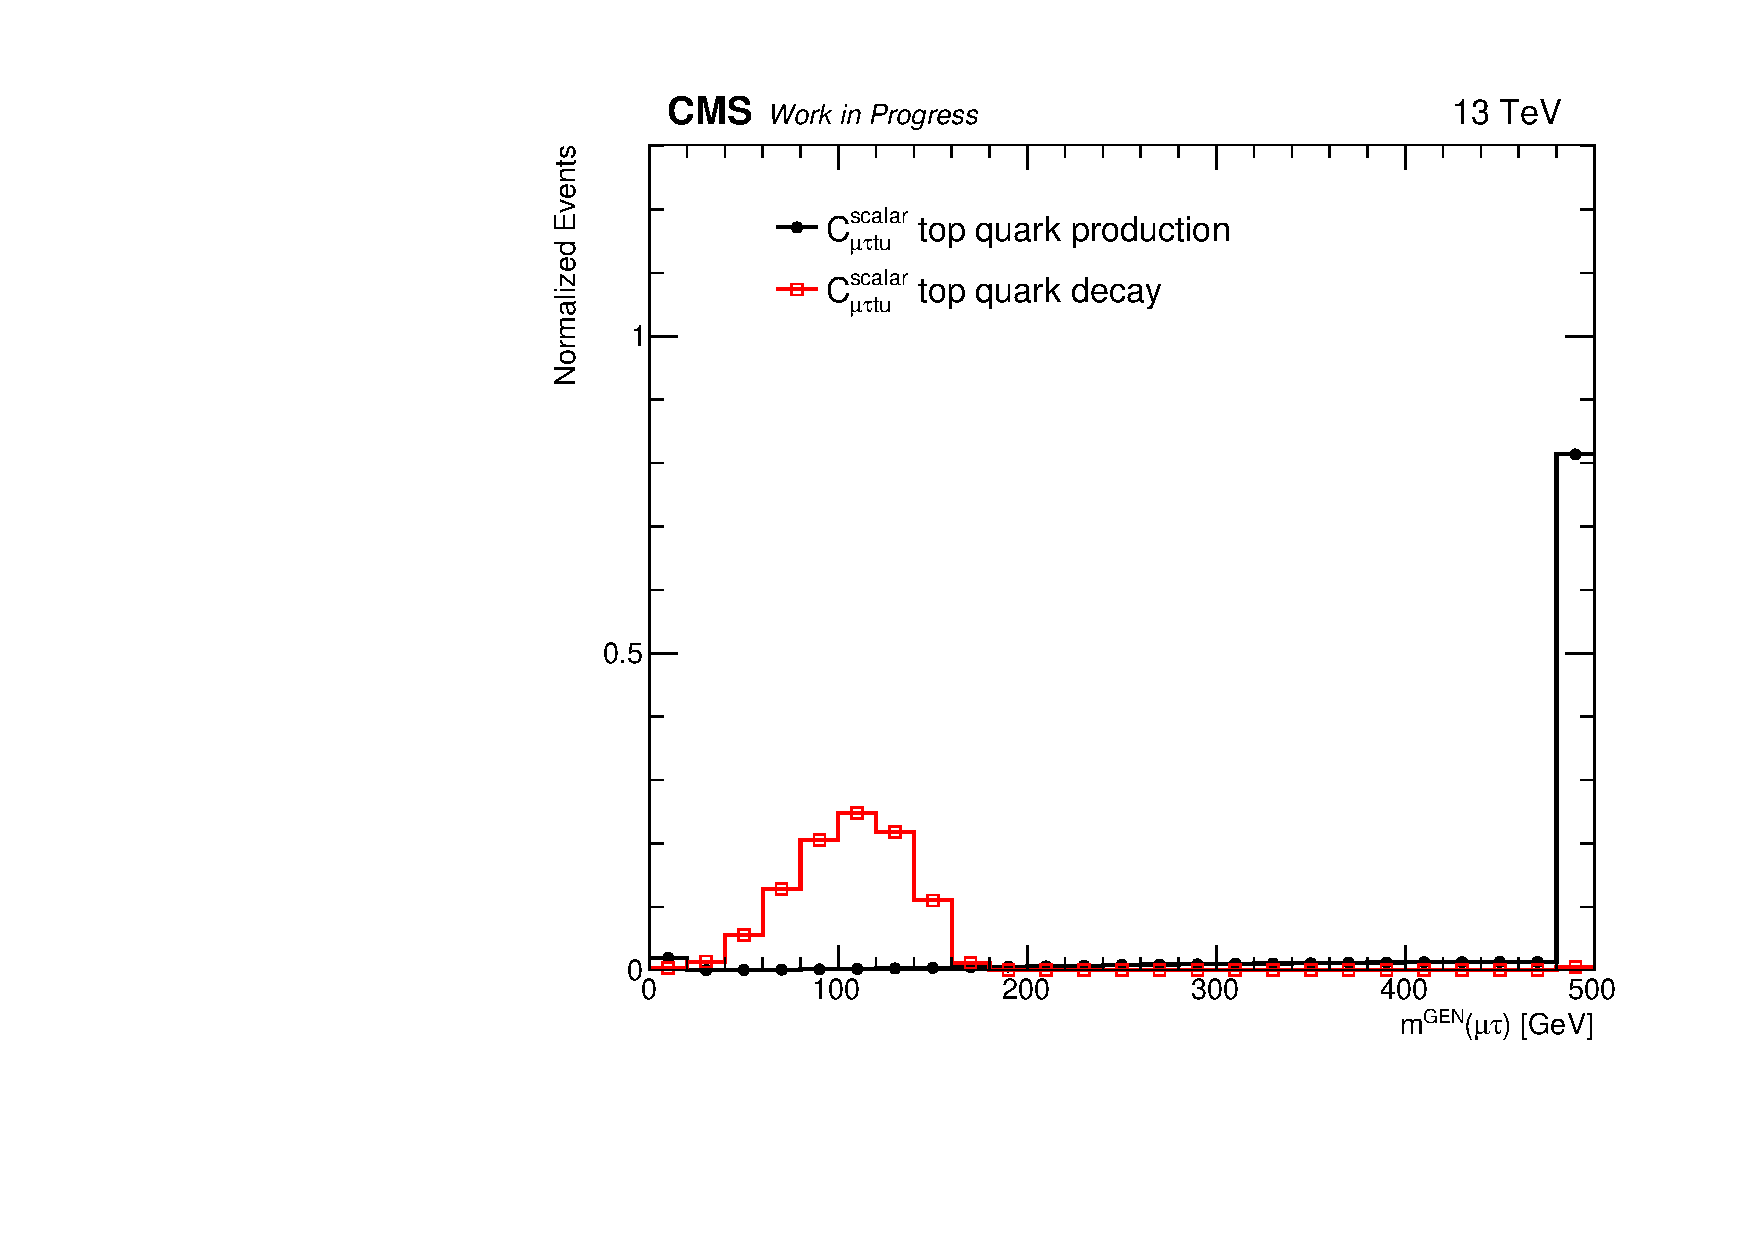
\includegraphics[width=0.33\textwidth]{figures/Part4/Signal/llM_mutau}\\
  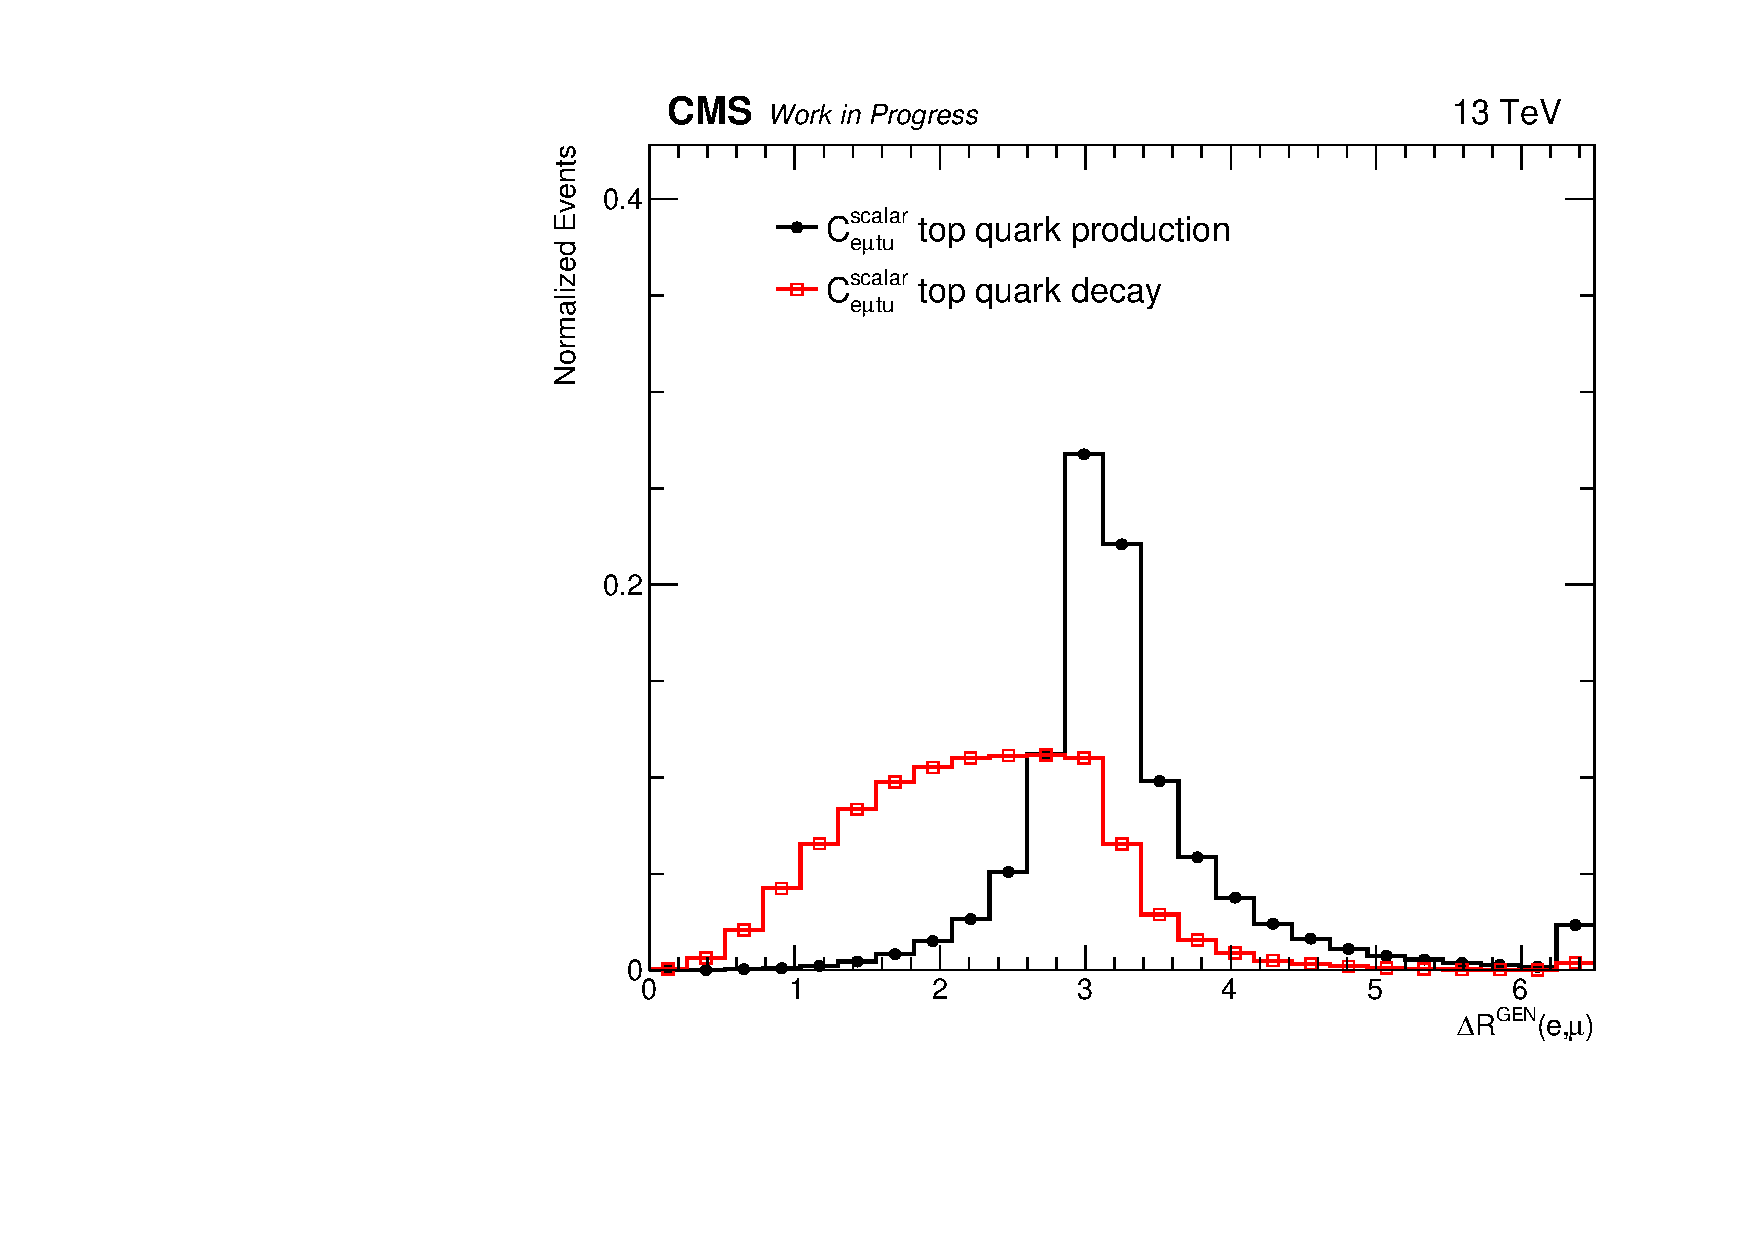
\includegraphics[width=0.33\textwidth]{figures/Part4/Signal/llDr_emu}&
 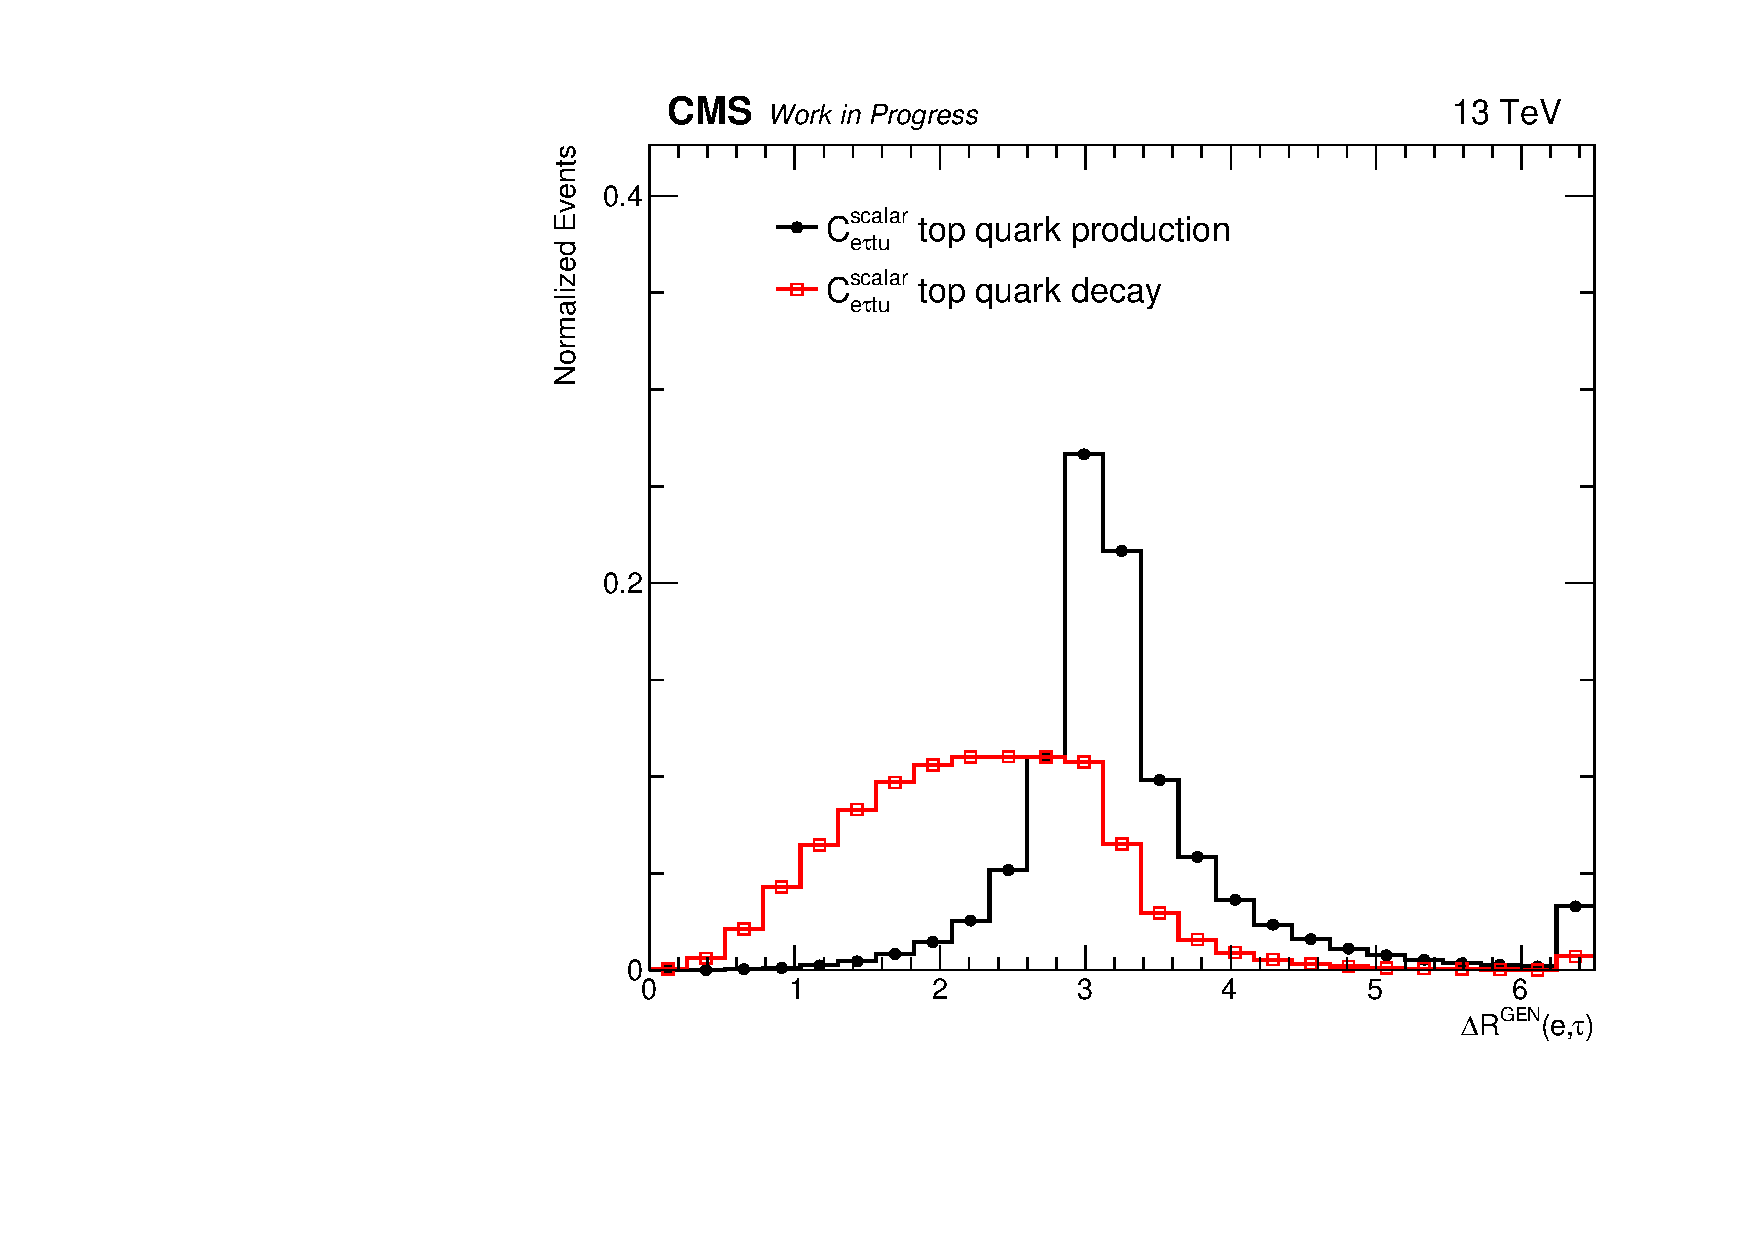
\includegraphics[width=0.33\textwidth]{figures/Part4/Signal/llDr_etau}&
 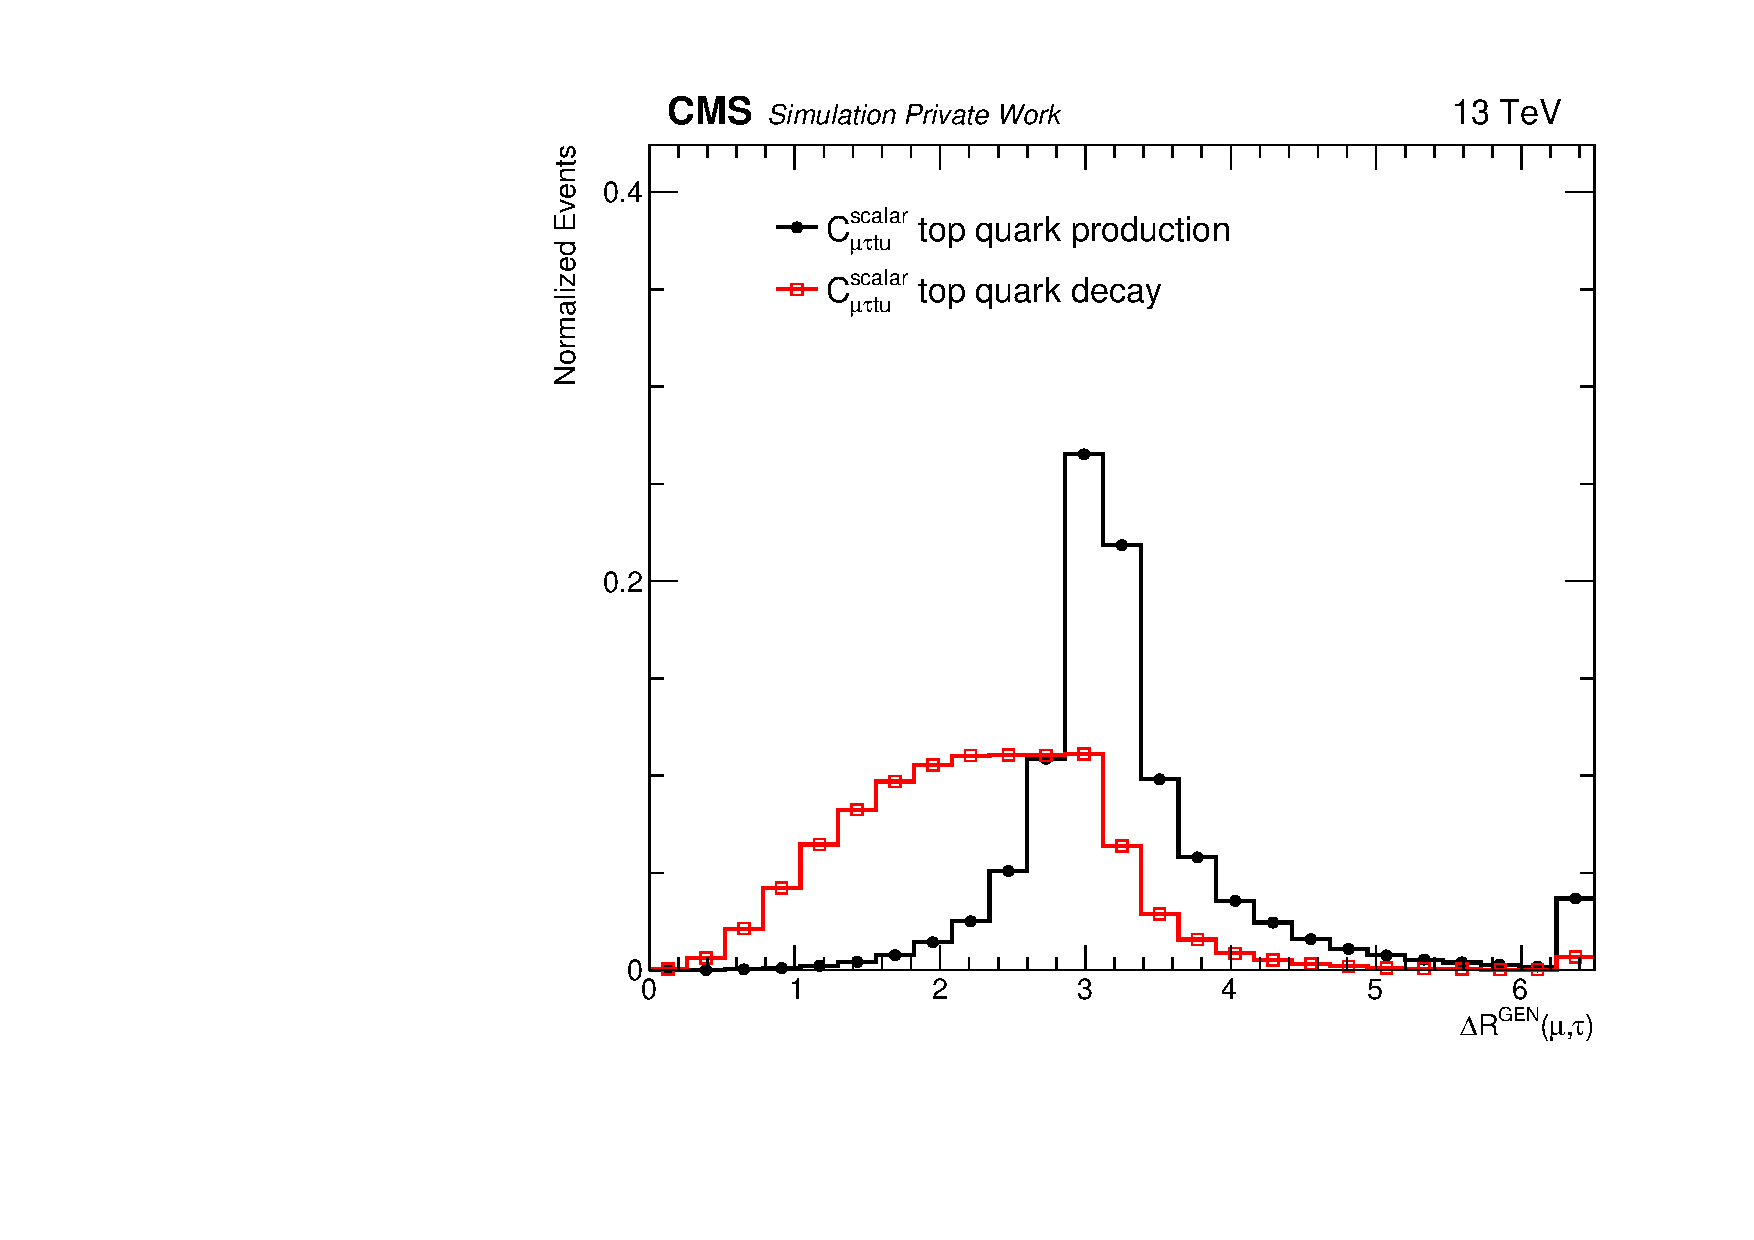
\includegraphics[width=0.33\textwidth]{figures/Part4/Signal/llDr_mutau}\\
 \end{tabular}
 \caption{Representative Feynman diagrams for the signal processes that are targeted by this analysis. Both top quark decay (left) and production (middle and right) \ac{CLFV} processes are shown. The indices $i$,  $j$, and $k$ are lepton flavor indices that run from 1 to 3 with the following conditions: i) $i\neq j$, ii) one of these three indices is 3, and iii) the other two are smaller than 3.}
 \label{fig:SigGen}
 \end{center}
 \end{figure}

